\section{Results}

\subsection{Clustering Evaluation}

The goal of this evaluation is to measure the accuracy of HDBSCAN, with different parameters and preprocessing methods. The most suitable settings will then be used for the online clustering approach to detect changes in a news stream.

\subsubsection{Setup}

\paragraph{Text Preprocessing}

 The first step in working with text is to apply Natural Language Processing techniques for improving the quality of the data before clustering it. We look the five different preprocessing methods as described in section \ref{sec:text_preprocessing} and evaluate each. The methods are:
 \begin{itemize}
     \item Full text with stop word removal
     \item Key terms
     \item Named entities
     \item Text lemmatisation
     \item Text stemming
 \end{itemize} 

\paragraph{Text Vectorization} Before the text can be clustered, it has to be transformed into a vector space model. We look at two different models:
\begin{itemize}
    \item Word Frequency
    \item tf-idf
\end{itemize}

\paragraph{Parameters} HDBSCAN has a range of parameters, which can be tuned to fit our data set. We focus on the two primary ones:
\begin{itemize}
    \item Min cluster size: The minimum size of a cluster. We run the evaluation with a range from two to nine as the $min\_cluster\_size$. 
    \item Metric: The distance measure between points. We apply the metrics "cosine" and "euclidean". 
\end{itemize}

The primary parameter for \textit{k}-means is the number of clusters. Since \textit{k}-means is used as a baseline to evaluate HDBSCAN, we provide the true number of clusters for each run. Therefore \textit{k}-means runs with an optimal starting point. 

\paragraph{Running the evaluation} The evaluation is done with different sets of news articles per run. This means if we define a run to use 30 stories and set it to repeat five times, each repeat will load 30 different stories from the data set. This is done to get a more diverse set of samples. Each run will be repeated at least five times. Lower numbers of stories allow for more repetitions due to lower processing times.   

\subsubsection{Evaluation}

The first run is done with 60 stories, which results in approximately 2000 news articles, over five repetitions. Table \ref{tab:cluster_parameters} shows the resulting MP-Score for each parameter in combination with each preprocessing method and vector space model. The highest score per parameter is highlighted as bold. The first insight we get  is the variety in scores for different min cluster sizes. The lowest min cluster size results in the lowest score, while increasing this parameter leads to an increasingly better score. The highest score is reached with a min cluster size of six, while increasing it further reduces the score again. The large difference in scores between different min cluster sizes, shows the importance this parameters has on the quality of the clustering and requires some knowledge of the data beforehand. In our case we have a wide range of different cluster sizes as shown in Figure \ref{fig:articles_per_story_distribution}, with clusters containing as few as two news articles. Based on this distribution we expected the ideal min size cluster size to be in a range from two to nine. The distribution also explains the drop in accuracy after a min cluster size of 6, since an increasingly number of clusters are being ignored.

\begin{table}[h]
    \centering
    \scalebox{0.65}{
    \begin{tabular}{|l|rrrrr|rrrrr|}
        \hline
        \textbf{Clustering} & \multicolumn{5}{ |c| }{\textbf{Word Frequency}} & \multicolumn{5}{ |c| }{\textbf{tf-idf}} \\
        \hline
        \textbf{HDBSCAN} & Full Text &  Key terms & Entities & Lemmatised & Stemmed & Full Text & Key terms & Entities & Lemmatised & Stemmed \\
        \hline
        min\_size: 2, metric: cosine    & 0.455 & 0.473 & 0.442 & 0.462 & 0.464 & 0.502     & 0.462 & 0.421 & \textbf{0.513} & 0.49      \\
        min\_size: 2, metric: euclidean & 0.066 & 0.064 & 0.089 & 0.068 & 0.068 & 0.422     & 0.240 & 0.457 & \textbf{0.461} & 0.445     \\
        min\_size: 3, metric: cosine    & 0.620 & 0.614 & 0.574 & 0.611 & 0.615 & 0.645     & 0.600 & 0.548 & \textbf{0.661} & 0.648     \\
        min\_size: 3, metric: euclidean & 0.067 & 0.063 & 0.091 & 0.067 & 0.067 & 0.554     & 0.267 & 0.553 & \textbf{0.584} & 0.573     \\
        min\_size: 4, metric: cosine    & 0.666 & 0.653 & 0.616 & 0.660 & 0.677 & 0.701     & 0.663 & 0.597 & 0.699     & \textbf{0.709} \\
        min\_size: 4, metric: euclidean & 0.059 & 0.059 & 0.083 & 0.058 & 0.059 & 0.576     & 0.273 & 0.574 & \textbf{0.600} & 0.595     \\
        min\_size: 5, metric: cosine    & 0.684 & 0.670 & 0.647 & 0.675 & 0.682 & 0.717     & 0.680 & 0.631 & 0.724     & \textbf{0.728} \\
        min\_size: 5, metric: euclidean & 0.046 & 0.054 & 0.081 & 0.049 & 0.049 & 0.567     & 0.266 & 0.582 & \textbf{0.605} & 0.602     \\
        min\_size: 6, metric: cosine    & 0.691 & 0.676 & 0.648 & 0.684 & 0.685 & 0.73      & 0.687 & 0.632 & 0.74      & \underline{\textbf{0.743}} \\
        min\_size: 6, metric: euclidean & 0.037 & 0.047 & 0.072 & 0.038 & 0.035 & 0.564     & 0.241 & 0.572 & \textbf{0.616} & 0.61      \\
        min\_size: 7, metric: cosine    & 0.690 & 0.673 & 0.640 & 0.680 & 0.688 & 0.737     & 0.691 & 0.632 & 0.737     & \textbf{0.739} \\
        min\_size: 7, metric: euclidean & 0.030 & 0.048 & 0.071 & 0.031 & 0.031 & 0.571     & 0.234 & 0.557 & \textbf{0.603} & 0.598     \\
        min\_size: 8, metric: cosine    & 0.674 & 0.667 & 0.633 & 0.669 & 0.678 & 0.727     & 0.679 & 0.625 & 0.728     & \textbf{0.729} \\
        min\_size: 8, metric: euclidean & 0.028 & 0.042 & 0.068 & 0.031 & 0.030 & 0.557     & 0.214 & 0.541 & \textbf{0.590} & 0.587     \\
        min\_size: 9, metric: cosine    & 0.669 & 0.663 & 0.625 & 0.657 & 0.669 & 0.715     & 0.672 & 0.623 & \textbf{0.728} & 0.724     \\
        min\_size: 9, metric: euclidean & 0.027 & 0.037 & 0.065 & 0.029 & 0.028 & 0.548     & 0.203 & 0.524 & \textbf{0.591} & 0.576     \\

        \hline
        \textbf{\textit{k}-means} & \multicolumn{5}{ |c| }{}  & \multicolumn{5}{ |c| }{} \\
        \hline
        n\_cluster: n\_true             & 0.375 & 0.418 & 0.276 & 0.354 & 0.365 & \textbf{0.638} & 0.622 & 0.478 & 0.634     & 0.636     \\
        \hline
    
    \end{tabular}   
    }
    \caption{The average MP-Score for combinations of parameter and preprocessing with a sample size of 60 stories (approx. 2000 articles)}
    \label{tab:cluster_parameters}
\end{table}

\begin{figure}[h]
    \centering
    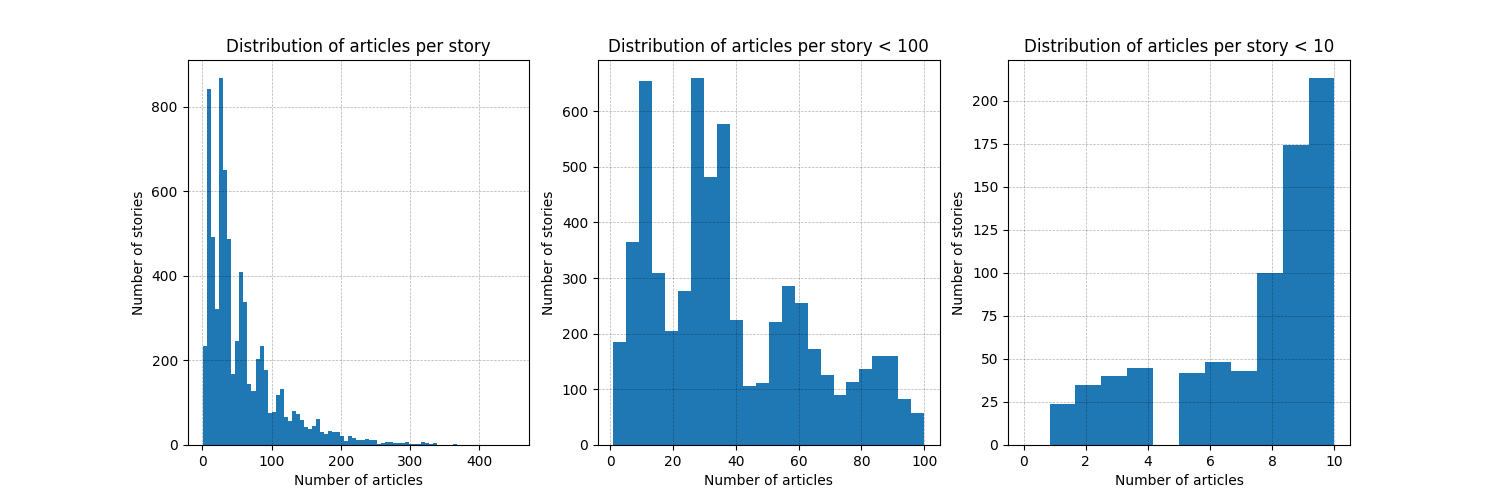
\includegraphics[width=1\textwidth]{articles_per_story_distribution}
    \caption{Distribution of cluster sizes.}
    \label{fig:articles_per_story_distribution}
\end{figure}

Comparing the two vector models, shows all of the best scores per parameter have been achieved by using tf-idf. Additionally the different metrics show a significant difference when using the vector model based on word frequency. With tf-idf the difference between both metrics is still notable, but far less drastic than based on word frequency. The overall better performance of the cosine metric over the euclidean distance is due to the high dimensionality and the sparseness of the vector space. This is behaviour has already been studied in the past\cite{Strehl00impactof}\cite{similarity_measures} and is one of the reasons, why the cosine similarity is often preferred over the euclidean distance as a similarity measure in the field of text mining.

As for the optimal preprocessing, text stemming provides the highest overall mp-score with 0.743, although closely followed by text lemmatization. This is to be expected, since both lemmatisation and stemming reduce the dimensions by grouping words into their base form, while still retaining most of the text.
In contrast to key term and entity extraction, which both result in a drastic reduction of the dimensions, and therefore less detail. It is also interesting to see how close the score from using the full text is compared to the best score per row. The difference between the overall best score of 0.743 achieved by stemming and the score provided by the full text of 0.73 is only 0.013. This means text preprocessing has a lesser impact than initially expected.   
However it is important to note, that we used pretrained models for key term and entity extraction.
Specifically training on a news corpus might improve the performance of both methods, but it was decided as to be out of scope for this thesis.

After determining the optimal settings for text preprocessing and vectorization, we increase the sample sizes for our evaluation runs, to get a deeper insight into the behaviour of HDBSCAN with larger data sets. Figure \ref{fig:hdbscan_parameters} shows the scores achieved with different parameters over an increasingly large set of samples. Based on this Figure we see the metric \textit{cosine} to be generally better than $euclidean$ and significantly more stable based on the range of the score and the quality of the clustering seems to decrease with larger sample sizes.

\begin{figure}[h]
    \centering
    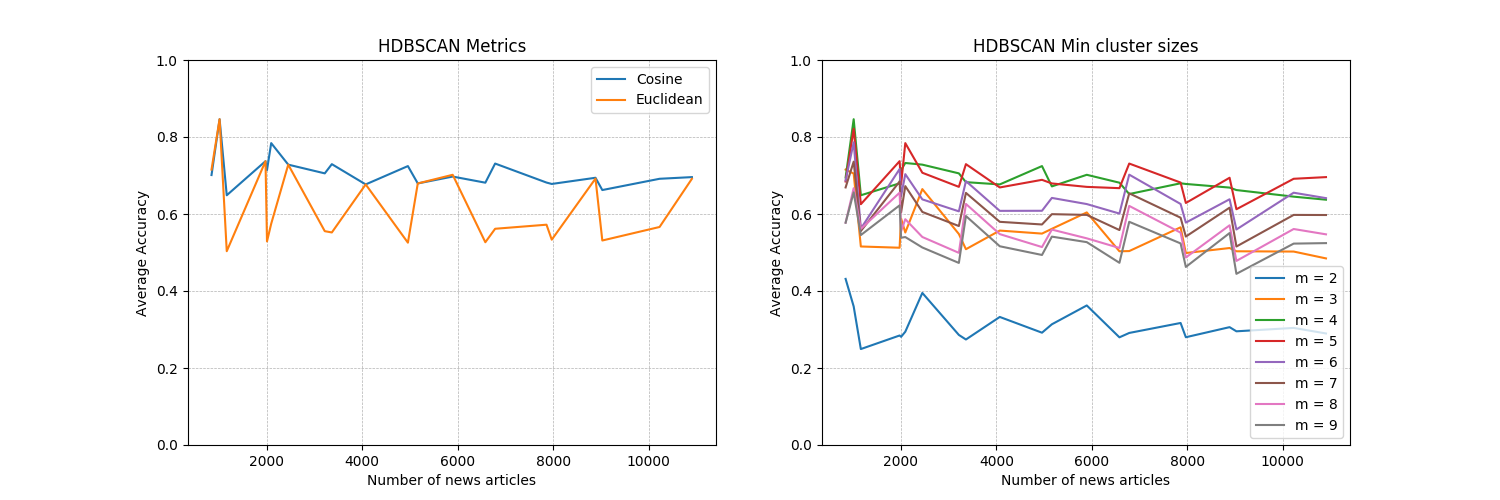
\includegraphics[width=1\textwidth]{hdbscan_parameters}
    \caption{MP-Score for different parameters, where min stands for the min cluster size. The marker represents the median, while the vertical line indicates the range between the min and max values. Each run contains at least five repetitions.}
    \label{fig:hdbscan_parameters}
\end{figure}

Furthermore the variance with smaller sample sizes can partially be explained through differences in the number of detected clusters, since missing a few clusters has a bigger impact if the overall number of clusters is small. Figure \label{fig:cluster_difference_samples} shows the difference between the number of predicted clusters and the number of true clusters. The Figure provides us with an interesting observation: While so far the minimum cluster size of six has given the best scores, the difference in the number of clusters is much smaller with a minimum cluster size of four. The MP-Score weights the similarity of a pair of clusters with their number of elements. This means ignoring smaller clusters has a lesser impact than ignoring larger clusters. We know our data set contains stories with news articles ranging from one up to 400. Based on this knowledge and the workings of the score, we can conclude that using a minimum cluster size of four gives us more clusters, which are ignored by using a larger minimum cluster size, but at the same time fragmenting larger clusters. Therefore resulting in a lower score, while having a better difference in the number of cluster predictions. This can be validated by analysing our data directly, where we observe the number of predicted cluster to be higher the lower the minimum cluster size is. Using $min\_cluster\_size=6$ tends to give a lower number compared the the true amount, while $min\_cluster\_size=3$ gives usually a higher number than there are actual clusters.

\begin{figure}[h]
    \centering
    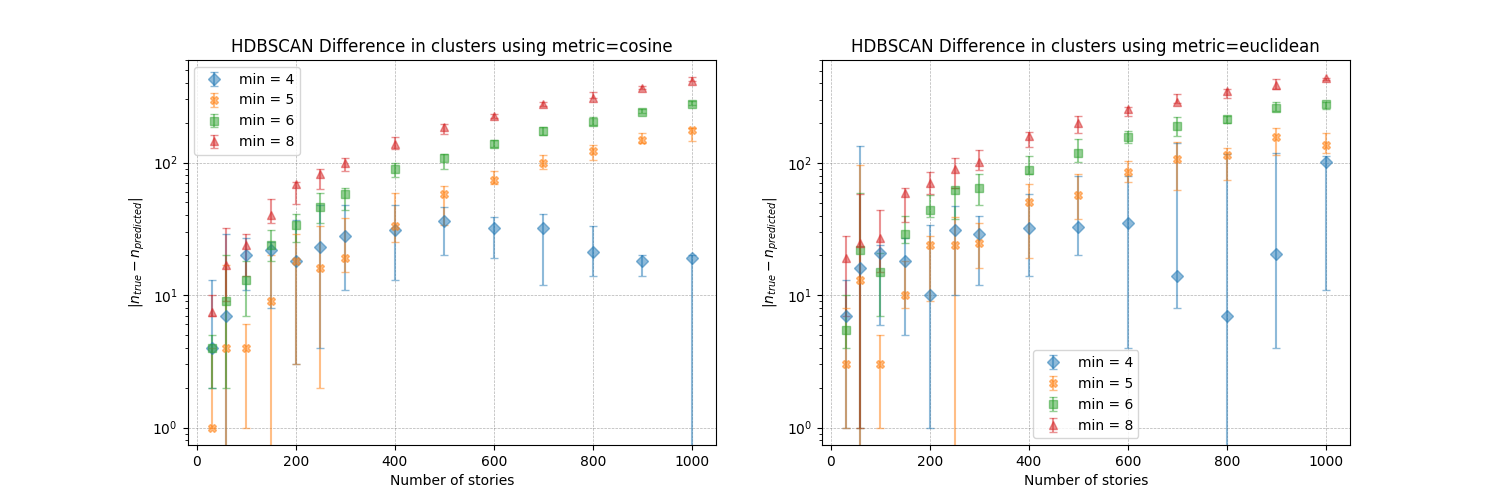
\includegraphics[width=1\textwidth]{cluster_differences}
    \caption{Difference between the predicted and true number of clusters.}
    \label{fig:cluster_differences}
\end{figure}

One of the advantages HDBSCAN has over other clustering algorithms, is the ability to work with noise, since we intent on applying it in an online setting, where noisy data is to be expected. At the same time, the number of articles classified as noise should be kept to a minimum. However the noise ratio shown in Figure \ref{fig:noise_ratio_samples} is significantly higher, than we would expect it to be based on our test data. A variety of factors play into the high noise ratio. One influence is due to the $min\_cluster\_size$. Each news article belonging to a cluster, which has less articles than the minimum cluster size, will be counted as noise. Table \ref{tab:expected_noise} lists the calculated percentage of news articles, which would be ignored based on different minimum cluster sizes. Although the percentages show that the impact the minimum cluster size has on the overall noise ratio is very limited. It is reasonably to assume, that the test data still contains a fair amount noisy data, even after cleaning up the data to the best of our efforts. Decreasing the noise ratio is certainly an important part in future improvements.

\begin{figure}[h]
    \centering
    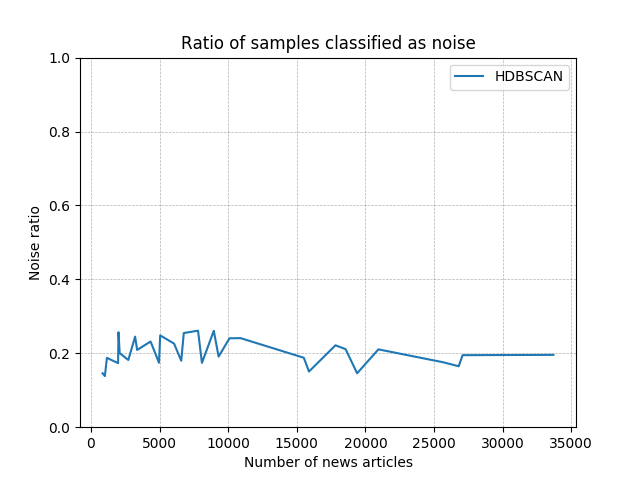
\includegraphics[width=1\textwidth]{noise_ratio_samples}
    \caption{Number of news articles classified as noise.}
    \label{fig:noise_ratio_samples}
\end{figure}

\begin{table}[h]
    \label{tab:expected_noise}
    \centering
    \begin{tabular}{|r|r|}
        \hline
        \textbf{min cluster size} & \textbf{Ignored articles} \\
        \hline
        2 & 0.032\% \\ \hline
        3 & 0.126\% \\ \hline
        4 & 0.304\% \\ \hline
        5 & 0.593\% \\ \hline
        6 & 0.985\% \\ \hline
        7 & 1.548\% \\ \hline
        8 & 2.168\% \\ \hline
        9 & 2.712\% \\ \hline
    \end{tabular}
    \caption{Percentages of ignored news articles because of their cluster size. The values are calculated directly based on the test data.}
\end{table}

% TODO hello saturday mile. Continue your work here 

Having determined the optimal settings to run HDBSCAN with, as text stemming with tf-idf, cosine as the similarity measure and six as the minimum size of clusters, we can start comparing the overall performance with \textit{k}-means. Figure \ref{fig:accuracy_kmeans_hdbscan} shows  a similar behaviour for both clustering methods in value and variance of the accuracy. Although HDBSCAN is generally more accurate than \textit{k}-means, the difference gets smaller with an increase in the sample size. Increasing the sample size results for both HDBSCAN and \textit{k}-means in a small loss regarding the accuracy as can be seen in Figure \ref{fig:accuracy_kmeans_hdbscan}. However the accuracy seems to stabilize around the 0.7 mark.

\begin{figure}[h]
    \centering
    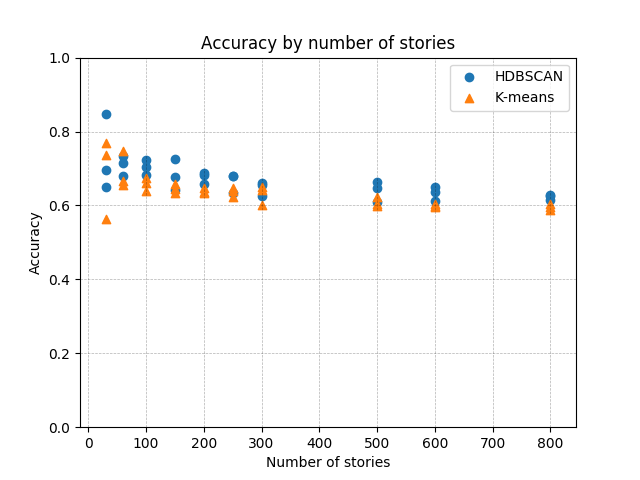
\includegraphics[width=0.5\textwidth]{accuracy_kmeans_hdbscan}
    \caption{Comparison of the average accuracy between \textit{k}-means and HDBSCAN}
    \label{fig:accuracy_kmeans_hdbscan}
\end{figure}

While HDBSCAN and \textit{k}-means provide a similar accuracy, the biggest difference can be noted in the processing time in relation to the number of samples. \textit{k}-means has a time complexity of $O(n^2)$ in contrast to HDBSCAN with a time complexity of $O(nlog(n))$, which is demonstrated by Figure \ref{fig:processing_time_kmeans_hdbscan}. Although running the evaluation has also shown the space complexity for HDBSCAN to be substantially higher for larger amounts of samples than with \textit{k}-means. Trying to run HDBSCAN with 100'000 news articles caused in a memory error, even with 64GB of RAM, while \textit{k}-means was able to complete the clustering.

% TODO measure memory?

\begin{figure}[h]
    \centering
    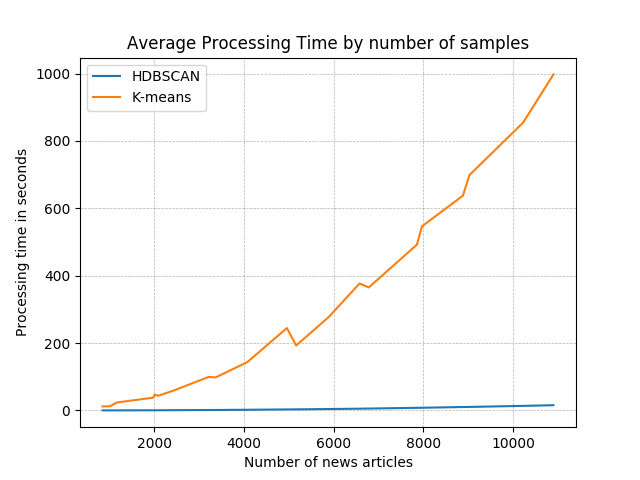
\includegraphics[width=0.5\textwidth]{processing_time_kmeans_hdbscan}
    \caption{Processing time in seconds }
    \label{fig:processing_time_kmeans_hdbscan}
\end{figure}


As a final note, we compare HDBSCAN with six different clustering methods taken from scikit-learn. Each method is run with a variety of parameters and the best scores are shown in Figure \ref{fig:different_clusterings}. HDBSCAN provides the highest accuracy, while being still being one of the fastest algorithms. Based on this data, we can assume HDBSCAN to be a good candidate for our use case.
% TODO rewrite
\begin{figure}[h]
    \centering
    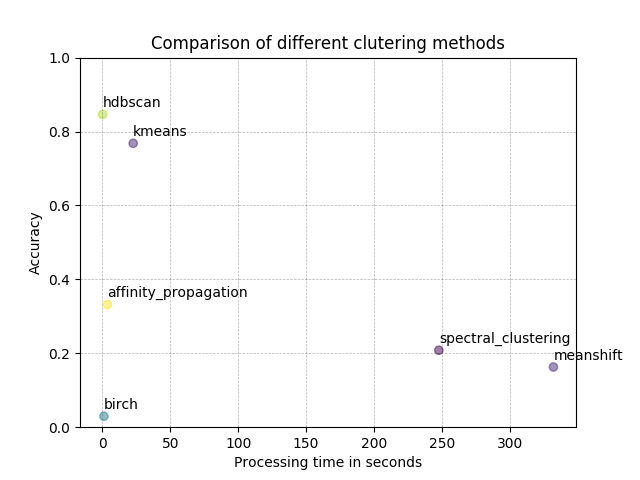
\includegraphics[width=0.5\textwidth]{different_clusterings}
    \caption{Comparison of different clustering methods with a sample size of approximately 1000 news articles}
    \label{fig:different_clusterings}
\end{figure}

\subsubsection{Conclusion}

The evaluation has shown HDBSCAN to be a good candidate to use for text based clustering. It provides an better accuracy than \textit{k}-means, while being significantly faster to process. The predicted number of clusters is consistent with an increasing number of samples and fairly close the truth. Additionally we have shown the required preprocessing and vectorization steps with the ideal parameters to achieve the most accurate results for our data set. However there is a substantial noise ratio, which causes almost a third of processed samples to be classified as noise. Another consideration is the space complexity  with larger data sets, where we quickly ran into issues we clustering over 50,000 samples. Overall HDBSCAN provides an acceptable accuracy, while still leaving room for further improvements.

\subsection{Online clustering}

\subsubsection{Setup}

The online clustering is done on a simulated stream of news articles based on the same data set as used in the clustering evaluation. This allows for direct comparison between the detected events and the ground truth. The settings to run the clustering are as follows:

\begin{itemize}
    \item Preprocessing: Text stemming
    \item Vector space model: tf-idf
    \item Clustering method: HDBSCAN
    \item Minimum cluster size: 6
    \item Distance metric: cosine
\end{itemize}

The clustering is run over 30 days with a total of 42'916 news articles. The distribution of news articles this time period is illustrated in Figure \ref{fig:news_articles_over_time}. The time delta, which is the amount of time between two batches, is set to one hour. 

\begin{figure}[h]
    \centering
    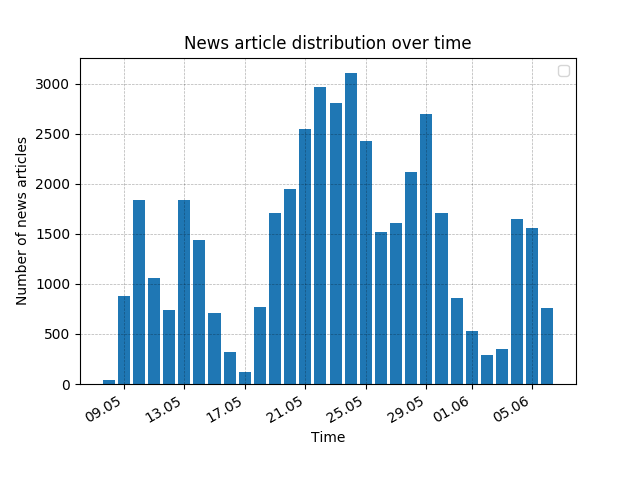
\includegraphics[width=0.5\textwidth]{news_articles_over_time}
    \caption{Incoming news articles over 30 days}
    \label{fig:news_articles_over_time}
\end{figure}

\subsubsection{Evaluation}

The goal of the online clustering is to detect new events in an incoming stream of news articles and changes in existing events. This evaluation analyses the results of our simulated test runs with different batch sizes.

Figure \ref{fig:event_detection_differences} shows the differences between the number of detected events and the number of true events for both new and existing topics. Based on this data we see the impact of different batch sizes for the accuracy in detected events. The difference with a batch size of 5000 news articles is significantly lower than the batch size of 1000. The difference is especially noticeable in the time period between the 21.05 and 25.05. The reason for this spike can be found in the distribution of incoming news articles as shown in Figure \ref{fig:news_articles_over_time}. During this period we receive up to 3000 news articles in a single day. This means by using a lower batch size such as 1000, the overlap between batches gets too small to reliably detect changes between batches, which causes too many new topics to be detected. 

\begin{figure}[h]
    \centering
    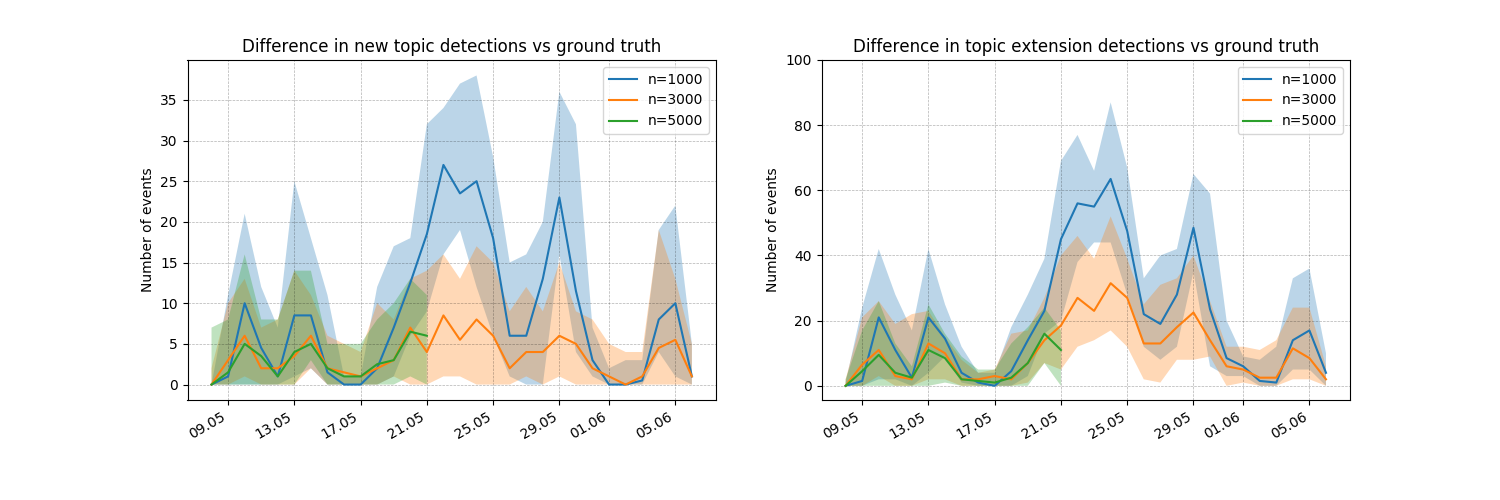
\includegraphics[width=1\textwidth]{event_detection_differences}
    \caption{Comparison between the difference in detected and true events. The line represents the median, while the area shows the range from the minimum to the maximum value}
    \label{fig:event_detection_differences}
\end{figure}

Although a larger batch size does not simply equal a better difference, as can be seen in Figure \ref{fig:event_detection_differences} by comparing the differences using a batch size of 3000 with a batch size of 5000. The batch size n=3000 shows a generally lower difference in the detection of new events than with n=5000. The differences between both batch sizes are less significant when detecting changes in existing events.

Based on the overall differences, we do not know the accuracy of those predictions. 
If the difference between newly detected events and true events is zero, there is still the possibility, that the events itself are different from the ground truth, and thus contain false positives. To measure the quality of events, we can look at the collection of events in a single batch as a subset of clusters, where each event is represented by a cluster containing all relevant news articles. Since we now have two clusterings, one containing detected events and the other with events taken from the ground truth, we can apply our MP-Score as a metric to get an insight into the quality of the detected events over the ground truth. Figure \ref{fig:event_detection_mp_score_1000} shows the MP-Scores for an online clustering using a batch size of 1000. Since there is quite a large variance, the score is shown as a boxplot, where a single box represents a full day. The large variance is already the first indication, that the quality is rather low. Meaning that there are still many false positives and false negatives.

\begin{figure}[h]
    \centering
    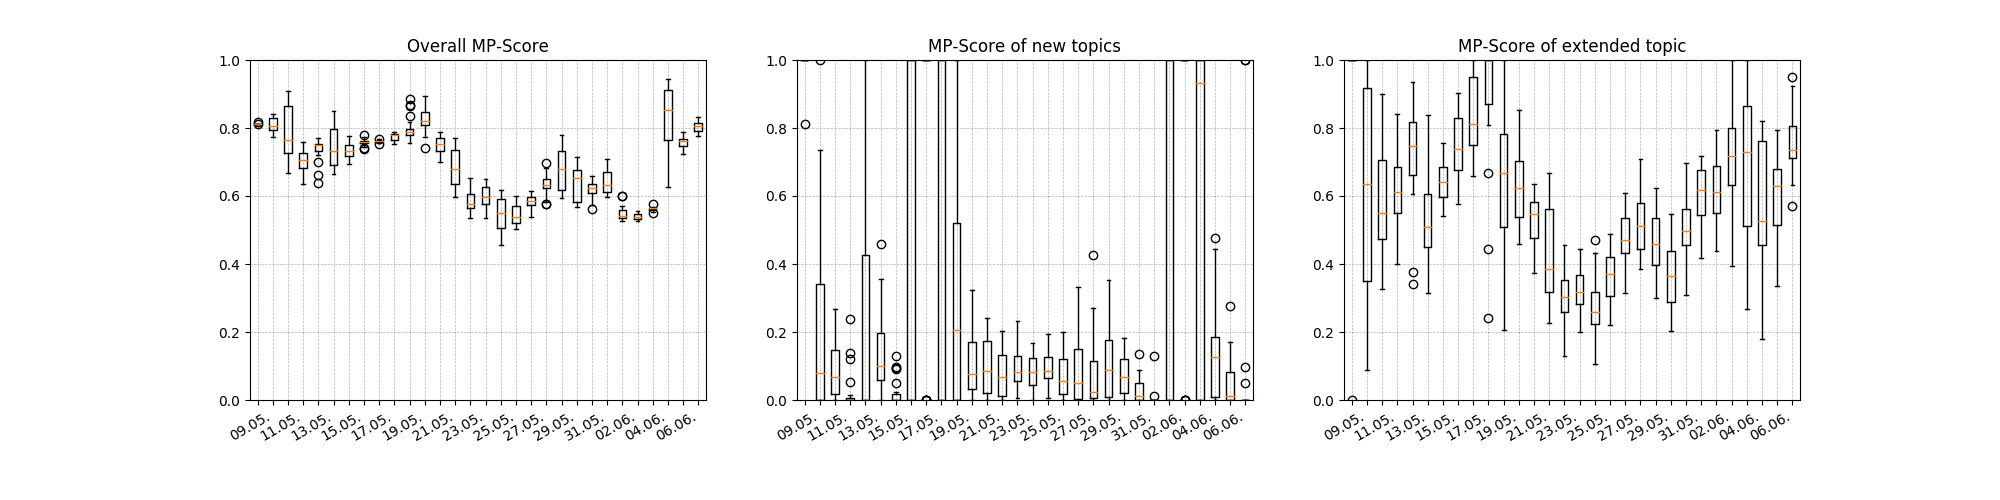
\includegraphics[width=1\textwidth]{event_detection_mp_score_1000}
    \caption{MP-Scores for clusterings using batch size of 1000}
    \label{fig:event_detection_mp_score_1000}
\end{figure}

Looking at an increased batch size of 5000 in Figure \ref{fig:event_detection_mp_score_5000}, we note that there is less variance in the overall MP-Score, which compares the full clustering with the ground truth. Although the variance for new and existing event detections is still fairly high. Additionally while the variance is high, the median for new topics is mostly around 0.1. This tells us that most of the newly detected events do not correspond with new events according to the ground truth. The detection of extensions of existing events is generally more accurate with a median between 0.5 and 0.8 using n=5000, but there is still are wide variance noticeable.

\begin{figure}[h]
    \centering
    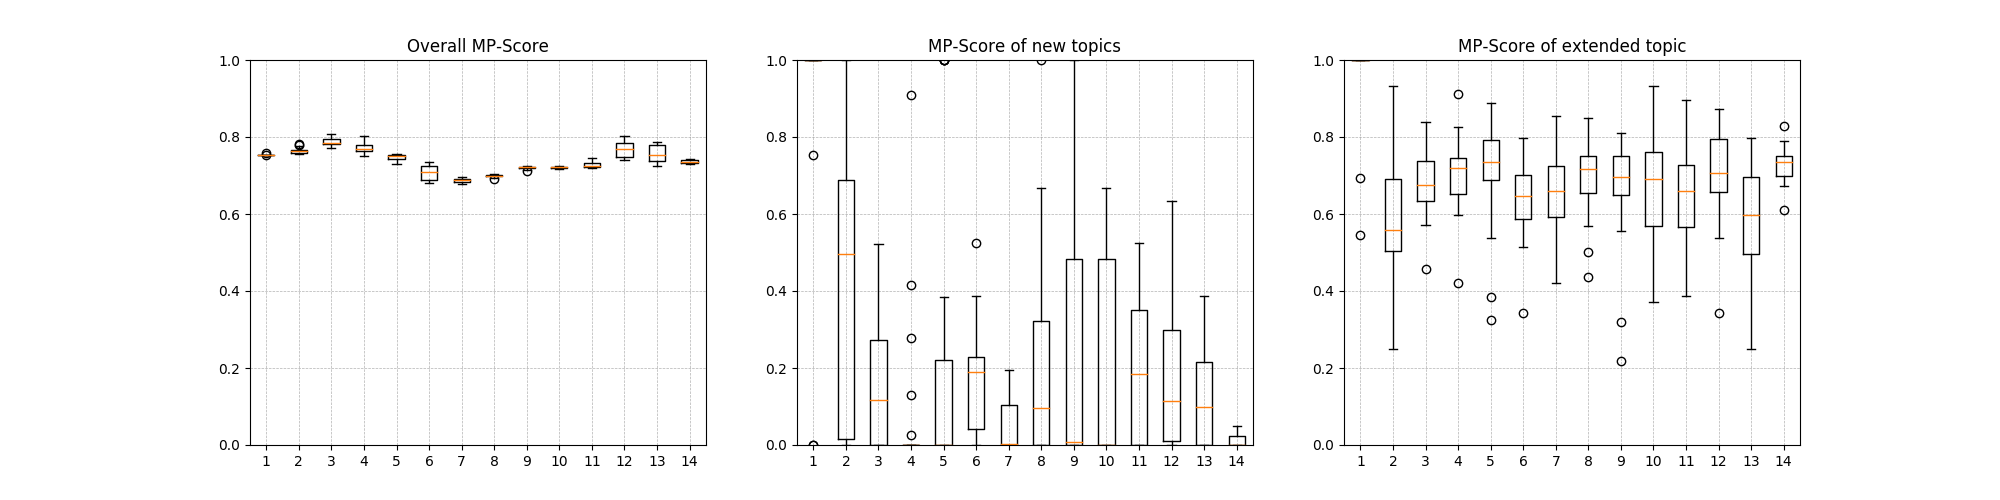
\includegraphics[width=1\textwidth]{event_detection_mp_score_5000}
    \caption{MP-Scores for clusterings using batch size of 5000}
    \label{fig:event_detection_mp_score_5000}
\end{figure}

One of the reasons for the difference in the accuracy of the detection of new events and the extension of events might be explained by the $min\_cluster\_size$. In the current setting the $min\_cluster\_size$ is set to 5, which means if an event occurs in batch one containing only four news articles, it will be discarded as noise. If the second batch contains additional news articles for the same event, it will be detected as a new occurrences, but the ground truth treats it as an existing event. To see how this affects the result we run the same simulation with a batch size of n=3000 a second time, but only considering new events from the ground truth if the number of news articles is greater or equal to the $min\_cluster\_size$.

\begin{figure}[h]
    \centering
    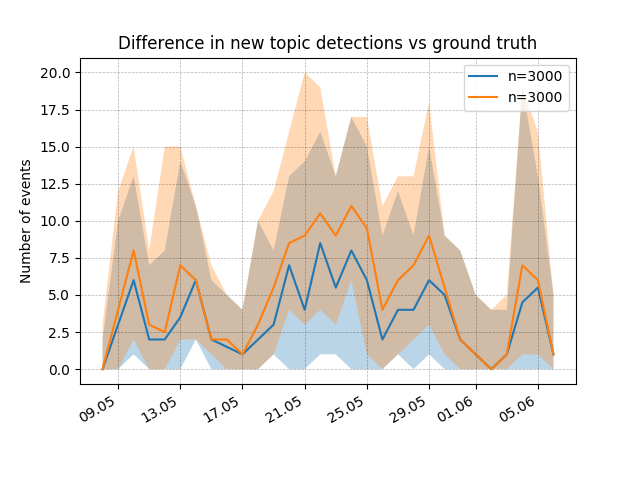
\includegraphics[width=0.5\textwidth]{event_detection_differences_with_min_cluster_size}
    \caption{Differences in predictions vs ground truth using batch size of 3000.}
    \label{fig:event_detection_differences_with_min_cluster_size}
\end{figure}

Limiting new events in the ground truth based on the $min\_cluster\_size$ gives the opposite result as initially expected. 
Figure \ref{fig:event_detection_differences_with_min_cluster_size} clearly shows an increase in the difference between predicted events and the adjusted ground truth. This means we already detected more new events than there were present in the ground truth and limiting it based on the $min\_cluster\_size$ only lowered the true number of events, thus leading to an increase in the difference. A look at the raw data from an initial simulation run in Figure \ref{fig:event_detection_by_date_3000} validates this assumption.

\begin{figure}[h]
    \centering
    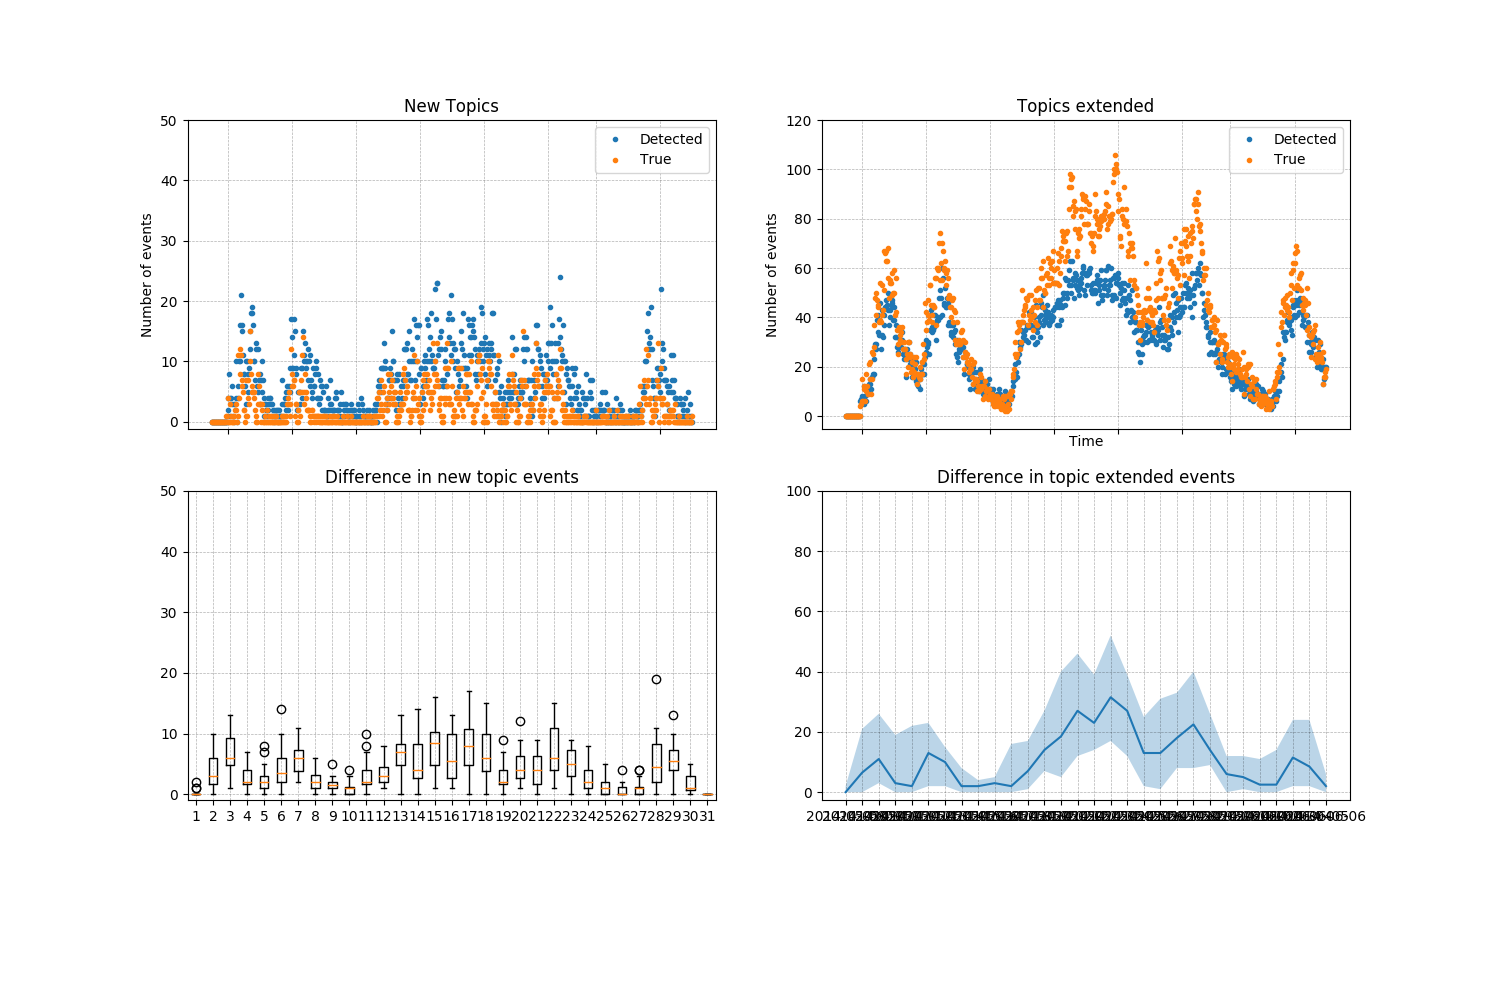
\includegraphics[width=1\textwidth]{event_detection_by_date_3000}
    \caption{Number of events with a batch size of 3000}
    \label{fig:event_detection_by_date_3000}
\end{figure}

The raw data in Figure \ref{fig:event_detection_by_date_3000} also shows a direct correlation between the number of detected new events and the number of detected changes in events. The more changes we missed, the more new events are detected. This is to be expected, since the detection of changes depends upon finding similar pairs of clusters in two different batches. If a cluster in the current batch could not be matched to a cluster from the previous batch, the cluster from the current batch will be seen as a new event. Therefore the accuracy in finding pairs of clusters in crucial to a better performance. The online clustering makes use of Locality Sensitive Hashing as explained in section \ref{sec:online_clustering_implementation}. The current threshold value for determining the similarity is set to 0.75. To see the impact on the similarity threshold, we run the online clustering again with a batch size of n=3000 and different threshold values.

\begin{figure}[h]
    \centering
    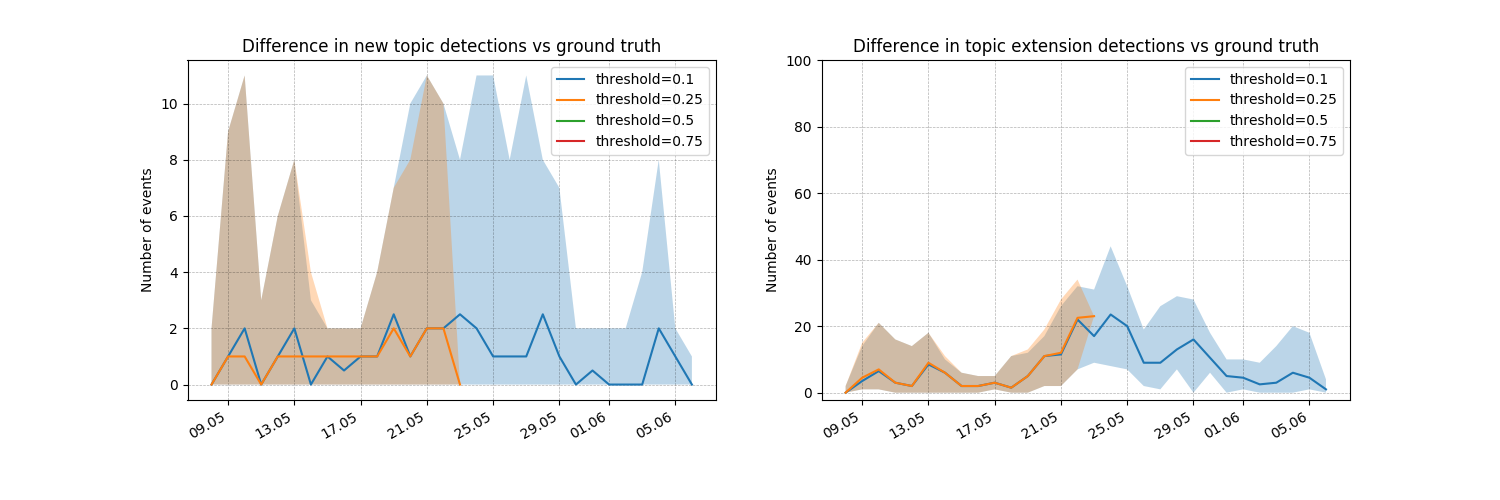
\includegraphics[width=1\textwidth]{event_detection_differences_threshold}
    \caption{Differences in detected over true events with different thresholds}
    \label{fig:event_detection_differences_threshold}
\end{figure}

Figure \ref{fig:event_detection_differences_threshold} shows the effect of the threshold on the difference in decided over true events. We see how the initial threshold of 0.75 was set too high, as lower threshold values such as 0.1 provide a significant lower difference. While there is still a substantial variance per day the median of 0.1 and 0.5 is generally more stable and lower than with a threshold value of 0.75. The reason for the better performance of lower threshold values, is that the overlap between batches decreases with an increase in the volume of news articles. This is clearly visible during the peaks in Figure \ref{fig:event_detection_differences_threshold}. Thus a high similarity threshold cannot be met, since there exists only an overlap of a few news articles for the same cluster between batches. The MP-Score is also improved for new events as can be seen in Figure \ref{fig:event_detection_mp_score_3000_0_1}. While there is more variance than in similar plots from Figure \ref{fig:event_detection_mp_score_1000} and Figure \ref{fig:event_detection_mp_score_5000}, the median from using threshold=0.1 clearly surpasses any measure from using threshold=0.75. The high variance in the boxplot is due to the fact, that there are only a few new events per hour, if any. This means detecting no events, when there are none leads to a score of 1, while detecting one event, when there is none leads to a score of 0.

\begin{figure}[h]
    \centering
    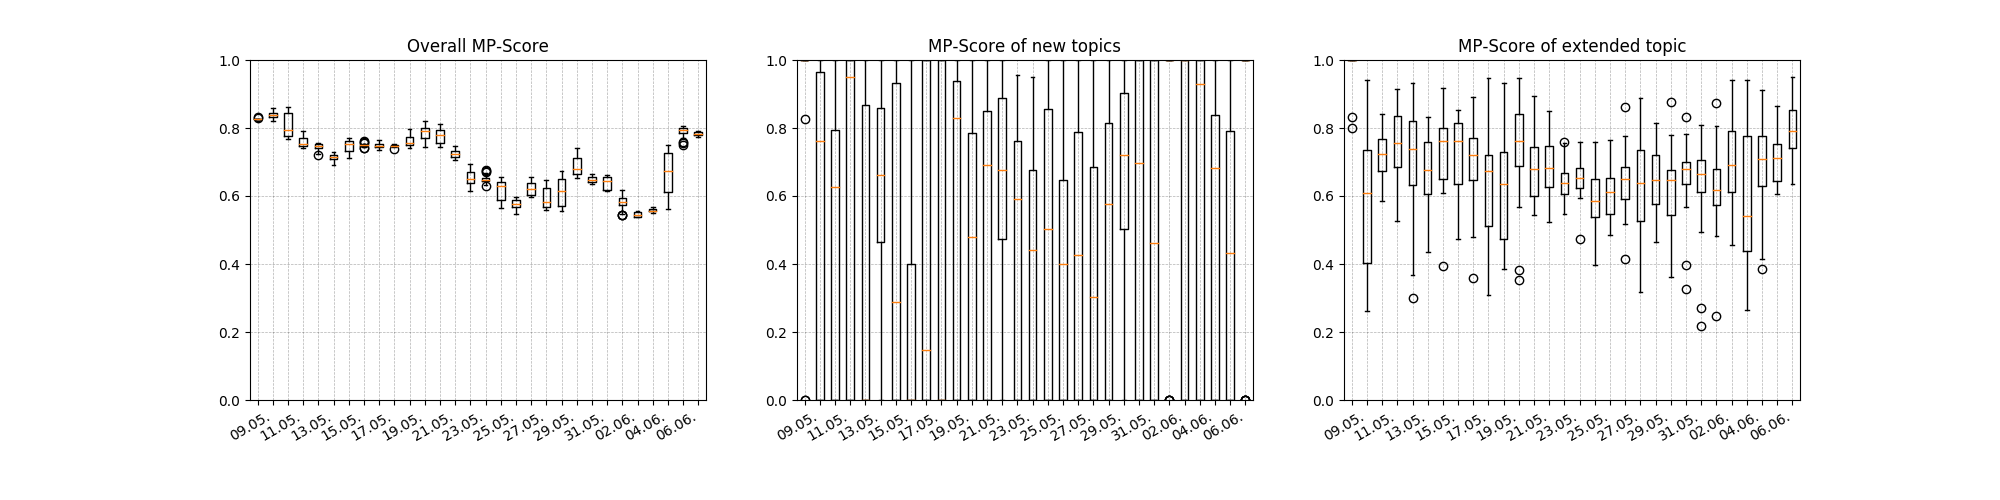
\includegraphics[width=1\textwidth]{event_detection_mp_score_3000_0_1}
    \caption{MP-Scores for online clustering with batch size n=3000 and threshold=0.1}
    \label{fig:event_detection_mp_score_3000_0_1}
\end{figure}


Additional reasons for the general low performance in the quality of events might be due to the noise rate and the difference in the number of news articles. As described in the section about the cluster method evaluation, the noise rate for sample sizes between 1000 and 5000 ranges from 20\% to 30\%. This means a significant amount gets discarded as noise and thus potential new events might not even be detected, because too many of their news articles are discarded. Once an event is detected, detection in changes are more reliable than for new events, but as the variance in the MP-Score shows, there is still a fairly large error rate.

% TODO how large?

As a final note let us look at two specific examples. One where the detection was mostly accurate and a second where the detection failed. Figure \ref{fig:online_clustering_example_gmail} shows the result for the story regarding the "Gmail redesign". Each dot represents one or more news articles, which appear at a certain time in the data stream. All news articles belong to the same story. As we can see after five news articles appearing in the stream, a new event is detected marked as green. Following the new event, additional news articles are clustered and detected as part of the existing event marked as blue. The last cluster does not contain all news articles any more, since the first few articles were not part of the last batch. However there is still enough overlap with the cluster from the previous batch, to match this cluster to the existing event about the "Gmail redesign". This example shows a good example of how the online clustering works in the optimal case.

\begin{figure}[h]
    \centering
    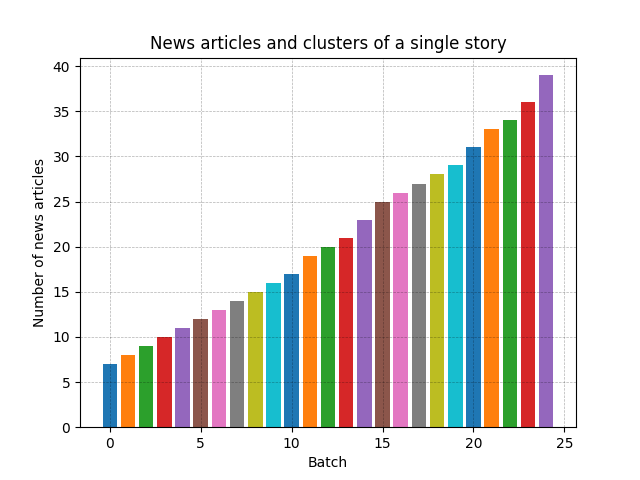
\includegraphics[width=1\textwidth]{online_clustering_example_gmail}
    \caption{News articles belonging to the story "Gmail redesign" together with clusters, where they appear in. The circles represent incoming news articles at a specific time. The rectangles show which news articles are contained within a cluster. New clusters are marked as green and existing cluster are blue.}
    \label{fig:online_clustering_example_gmail}
\end{figure}

The second example shown in Figure \ref{fig:online_clustering_example_neighbours} illustrates the opposite case, where the events do not match well with the ground truth. All news articles in this example belong to a story about the release of new film called "Bad Neighbours". Black dots indicate news articles, which do not appear in any cluster. The fragmentation of the clusters themselves clearly shows, that many of these news articles have been matched with different stories and therefore in different events. 

\begin{figure}[h]
    \centering
    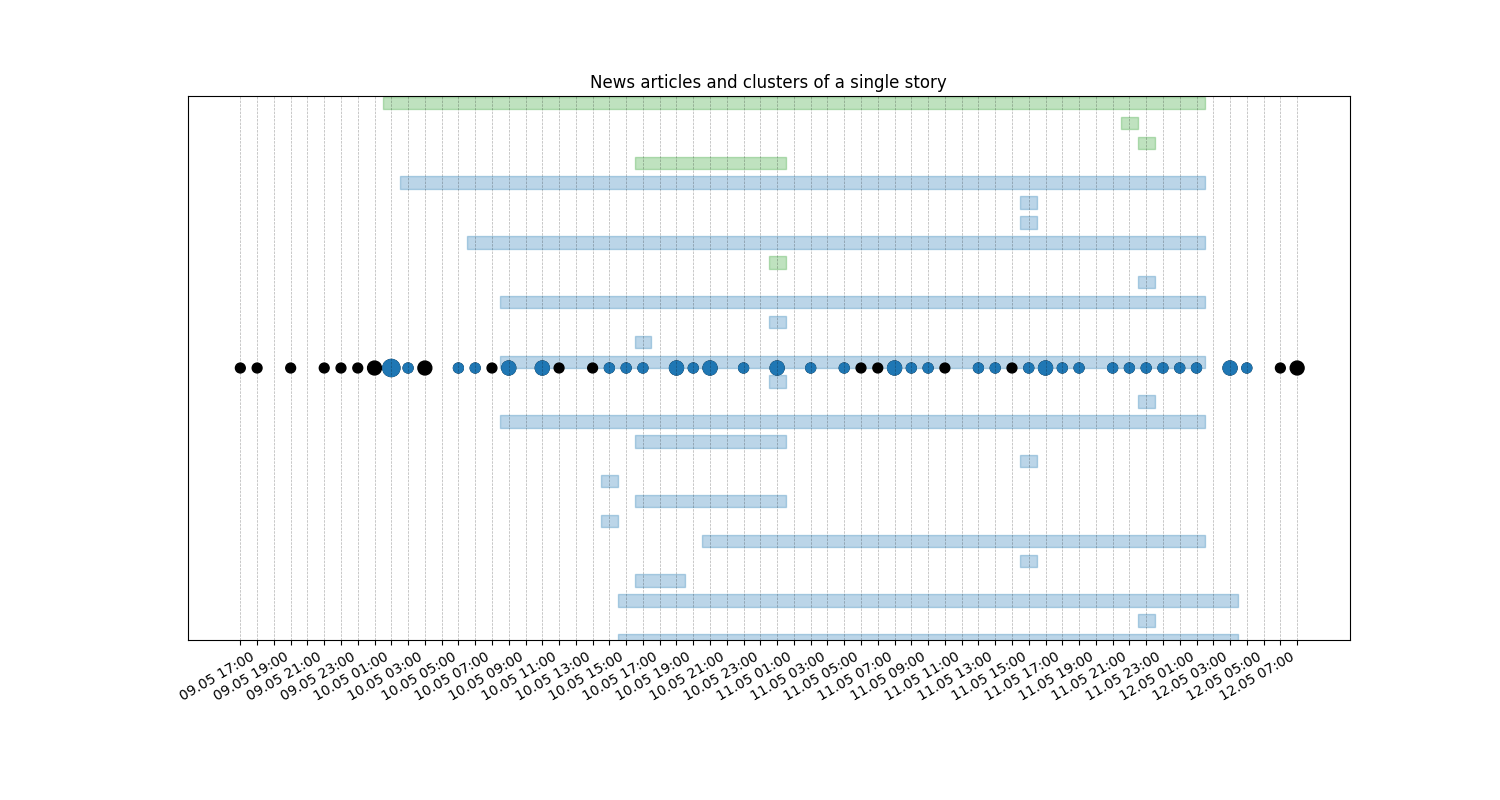
\includegraphics[width=1\textwidth]{online_clustering_example_neighbours}
    \caption{News articles belonging to the story "Bad Neighbours" together with clusters, where they appear in. Circles marked as black represent news articles, which do not appear in any cluster.}
    \label{fig:online_clustering_example_neighbours}
\end{figure}

The difference in the performance of both examples, can be explained based on the news articles themselves. The first example about the "Gmail redesign" consists mostly of press releases, technology focused news sites such as \textit{Ars Technica} or \textit{PC Magazine}. Therefore the contents of the news articles are of high quality and share the same technical vocabulary. The second example with the new release of the movie "Bad Neighbours" has a wider variety of sources and types of articles. Some news articles are short summaries, while others are interviews or personal reviews. Additionally the vocabulary is more general than compared to technical articles. 

\subsubsection{Conclusion}

TODO rewrite with new findings e.g. not as bad as initially thought but still not very good.

While the overall clustering results in good scores, the detection of new events and changes in existing events gives rather poor results. Possible reasons have been explored such as the $min\_cluster\_size$, the noise rate or the general difference in the number of news articles, but there exist no simple solutions for any of them. As a result we conclude that the accuracy of the clustering method used in this approach is insufficient for the detection of events in a news stream. TODO elaborate a bit more